
%\documentstyle[epsf,twocolumn]{jarticle}       %LaTeX2.09仕様
%\documentclass[twocolumn]{jarticle}     %pLaTeX2e仕様
\documentclass{jarticle}     %pLaTeX2e仕様

%一枚組だったら[twocolumn]関係のとこ消す

\setlength{\topmargin}{-45pt}
%\setlength{\oddsidemargin}{0cm} 
\setlength{\oddsidemargin}{-7.5mm}
%\setlength{\evensidemargin}{0cm} 
\setlength{\textheight}{24.1cm}
%setlength{\textheight}{25cm} 
\setlength{\textwidth}{17.4cm}
%\setlength{\textwidth}{172mm} 
\setlength{\columnsep}{11mm}

\kanjiskip=.07zw plus.5pt minus.5pt

\usepackage{graphicx}
\usepackage[dvipdfmx]{color}
\usepackage{subcaption}
\usepackage{enumerate}
\usepackage{comment}
\usepackage{url}
\usepackage{multirow}
\usepackage{diagbox}
\usepackage{amsmath,amssymb}
\usepackage{mathtools}
\usepackage{wrapfig}
\usepackage{graphicx}
\usepackage{float}



\begin{document}
  \noindent
  \onecolumn
  \hspace{1em}

  \today
  \hfill
  \ \ B3 西村昭賢 

  \vspace{2mm}
  \hrule
  \begin{center}
  {\Large \bf 進捗報告}
  \end{center}
  \hrule
  \vspace{3mm}


\section{今週やったこと}
\begin{quote}
  \begin{itemize}
   \item 学習ステップ数を増やした DQN の結果
   \item DQN の実験の結果を踏まえた改善
   \item DQN の再実験
   \item コスト, HP ,特殊効果追加した ver の環境の作成
  \end{itemize}
 \end{quote}


\section{学習ステップを増やした DQN の実験結果}
先週, DQN で 200000 ステップ(約 5000 エピソード)学習した結果先手が勝率 5 割を切るという結果となった.一方, 新たに実装したモンテカルロ探索では 1000000 エピソード学習し先手で 0.8011 という勝率を残した.\par
この結果を受け, DQN のステップ数を増やして学習が行われるか実験した.パラメータは表 \ref{table:param} に示す.
\begin{table}[h]
  \centering
  \caption{DQNのパラメータ}
  \label{table:param}
  \begin{tabular}{|c||c|}
  \hline
  方策                 & ε-greedy \\ \hline
  ε                      & 0.1      \\ \hline
  全結合層の活性化関数             & ReLU     \\ \hline
  全結合層の次元                & 64       \\ \hline
  最適化アルゴリズム              & Adam     \\ \hline
  Target Network 更新重み               & 1e-2     \\ \hline
  Experience Replayのメモリ量 & 1000000  \\ \hline
  \end{tabular}
  \end{table}

結果, 10000000ステップ先手で学習し,勝率は 0.3631 となった.学習の過程を図 \ref{fig:10000000} に示す.
全く学習できてないので環境側の問題,モデル側の問題の2つに分けて改善を図った.
\begin{figure}[H]
  \centering
  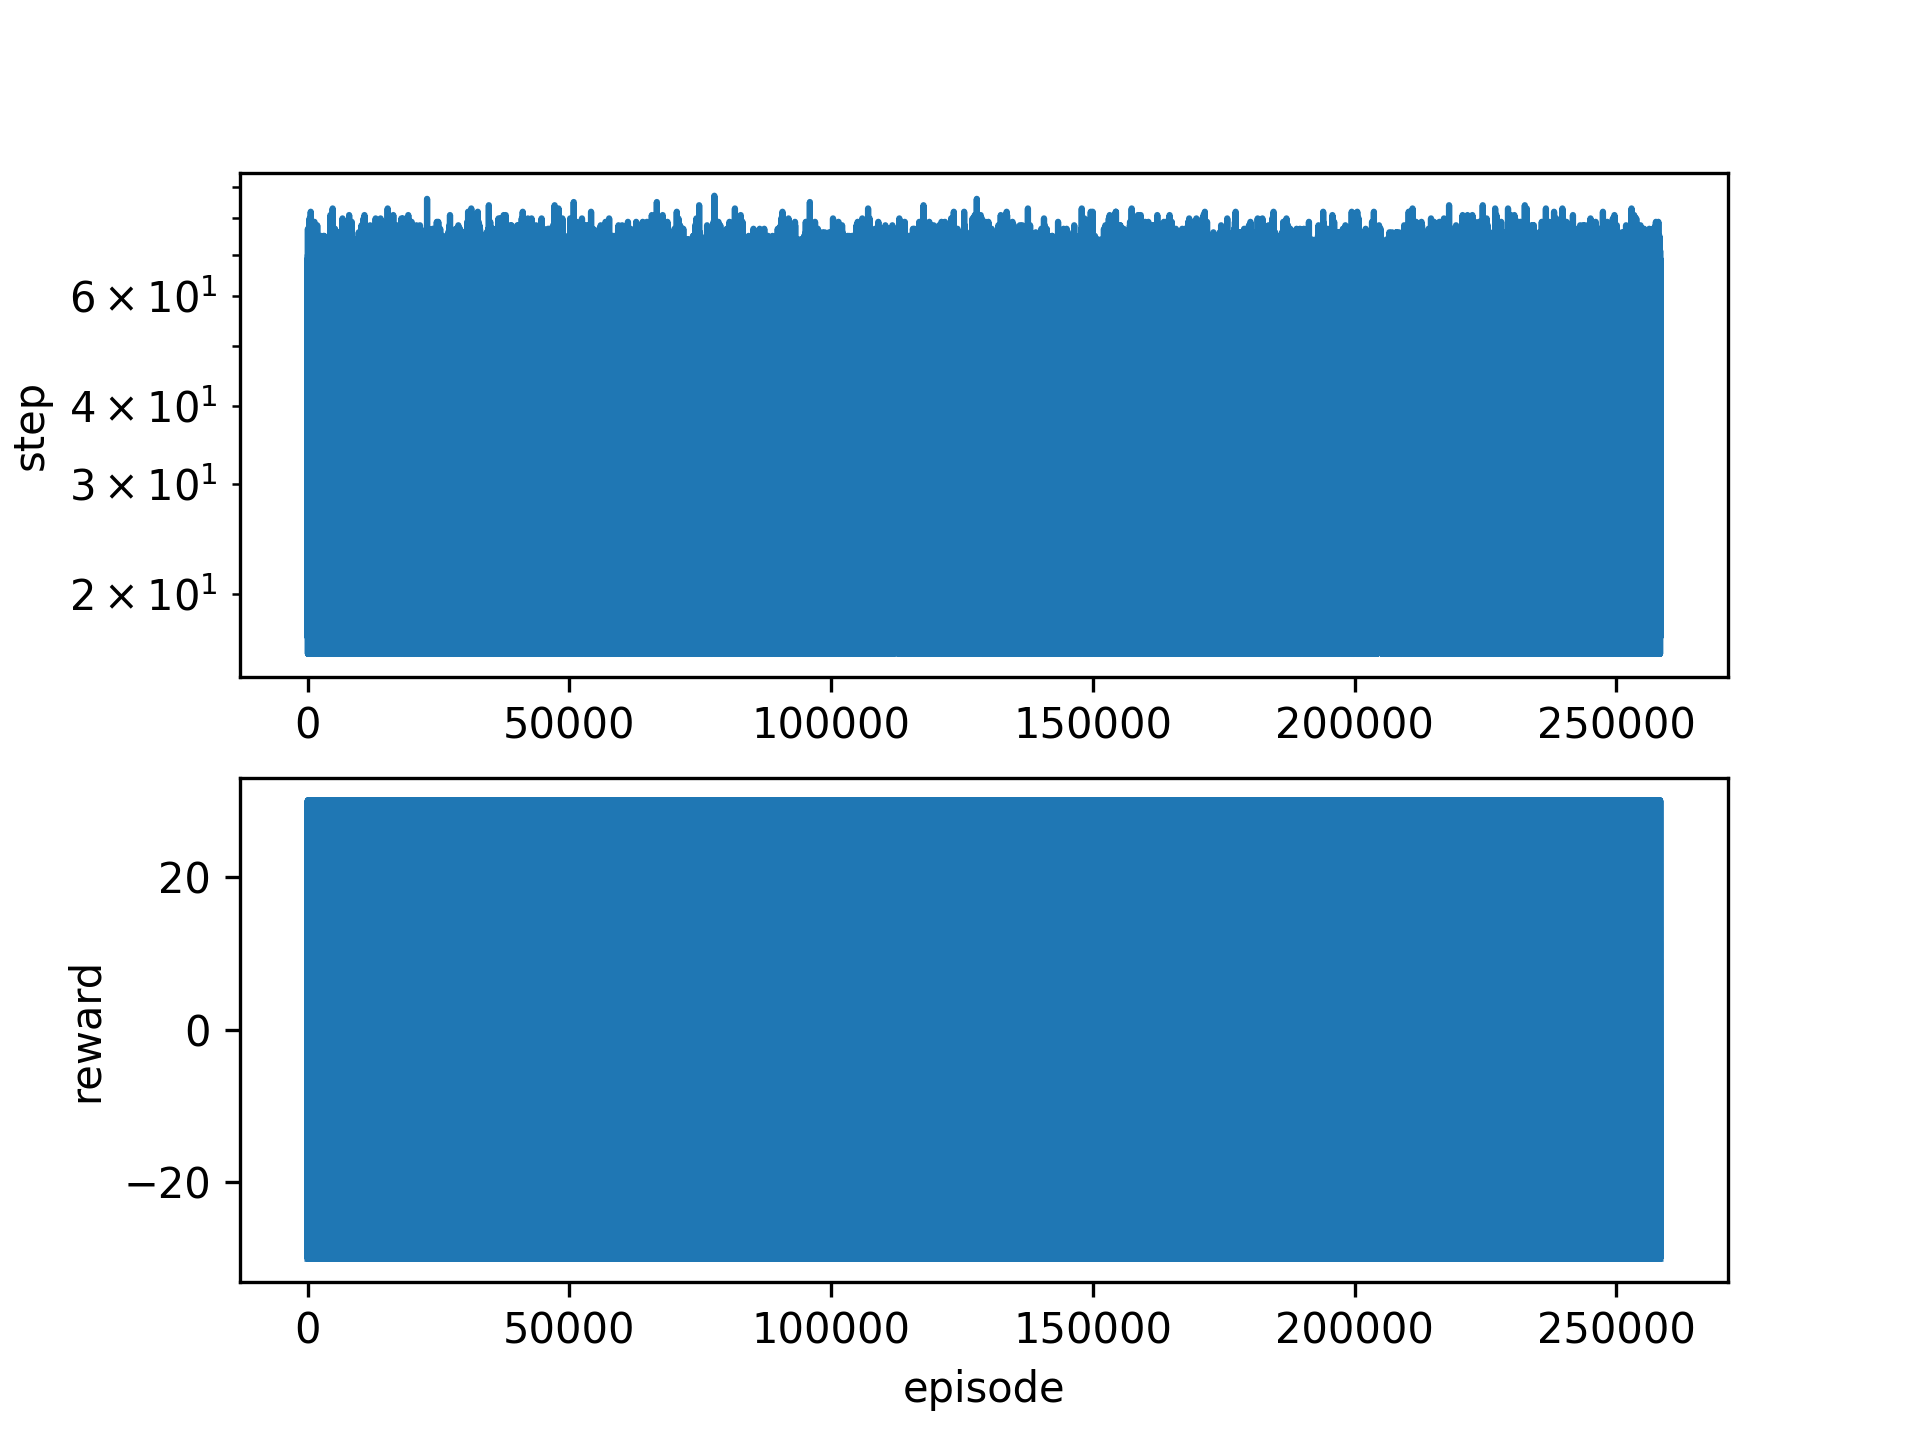
\includegraphics[width=120mm]{assets/10000000.eps}
  \caption{10000000 ステップの学習結果}
  \label{fig:10000000}
\end{figure}


\section{DQN の実験の結果を踏まえた改善}
\subsection{環境側の改善}
以下のような改善を図った.
\begin{quote}
  \begin{itemize}
  \item ライブラリを変更
   \item 行動空間の定義の変更
   \item 終了条件の変更
   \item 報酬の変更
   \item 状態空間の定義の変更
  \end{itemize}
 \end{quote}

\subsubsection{ライブラリ変更}
学習プレイヤーと敵プレイヤーのライブラリを表 \ref{table:deck} のようにして同じライブラリにした.
\begin{table}[H]
  \centering
  \caption{ライブラリ ()内の数字は(攻撃力, HP)を表す}
  \label{table:deck}
  \begin{tabular}{|c|c|}
  \hline
  カード   & 枚数 \\ \hline
  (3,3) & 5  \\ \hline
  (2,4) & 5  \\ \hline
  (2,3) & 5  \\ \hline
  \end{tabular}
  \end{table}

\subsubsection{行動空間の変更}
以前は「自盤面のターン中に行動可能なカードが全て行動すると自動的にターンエンド」としていた.上手く行かない学習過程を見てみると,盤面にカードが存在しない時にこの条件では1枚カードをプレイして強制的にターンエンドとなってしまっていることに気づいた.\par
この問題を解決するために手札のカードに対しても表 \ref{table:action} に示すように「プレイしない」という選択肢をつけて,「自手札,自盤面全てのカードについてターン中に何をするか決定したら自動的にターンエンド」と条件を変更した.\par

ゲームのイメージは図 \ref{fig:env}の通り変更はない.

\begin{figure}[H]
  \centering
  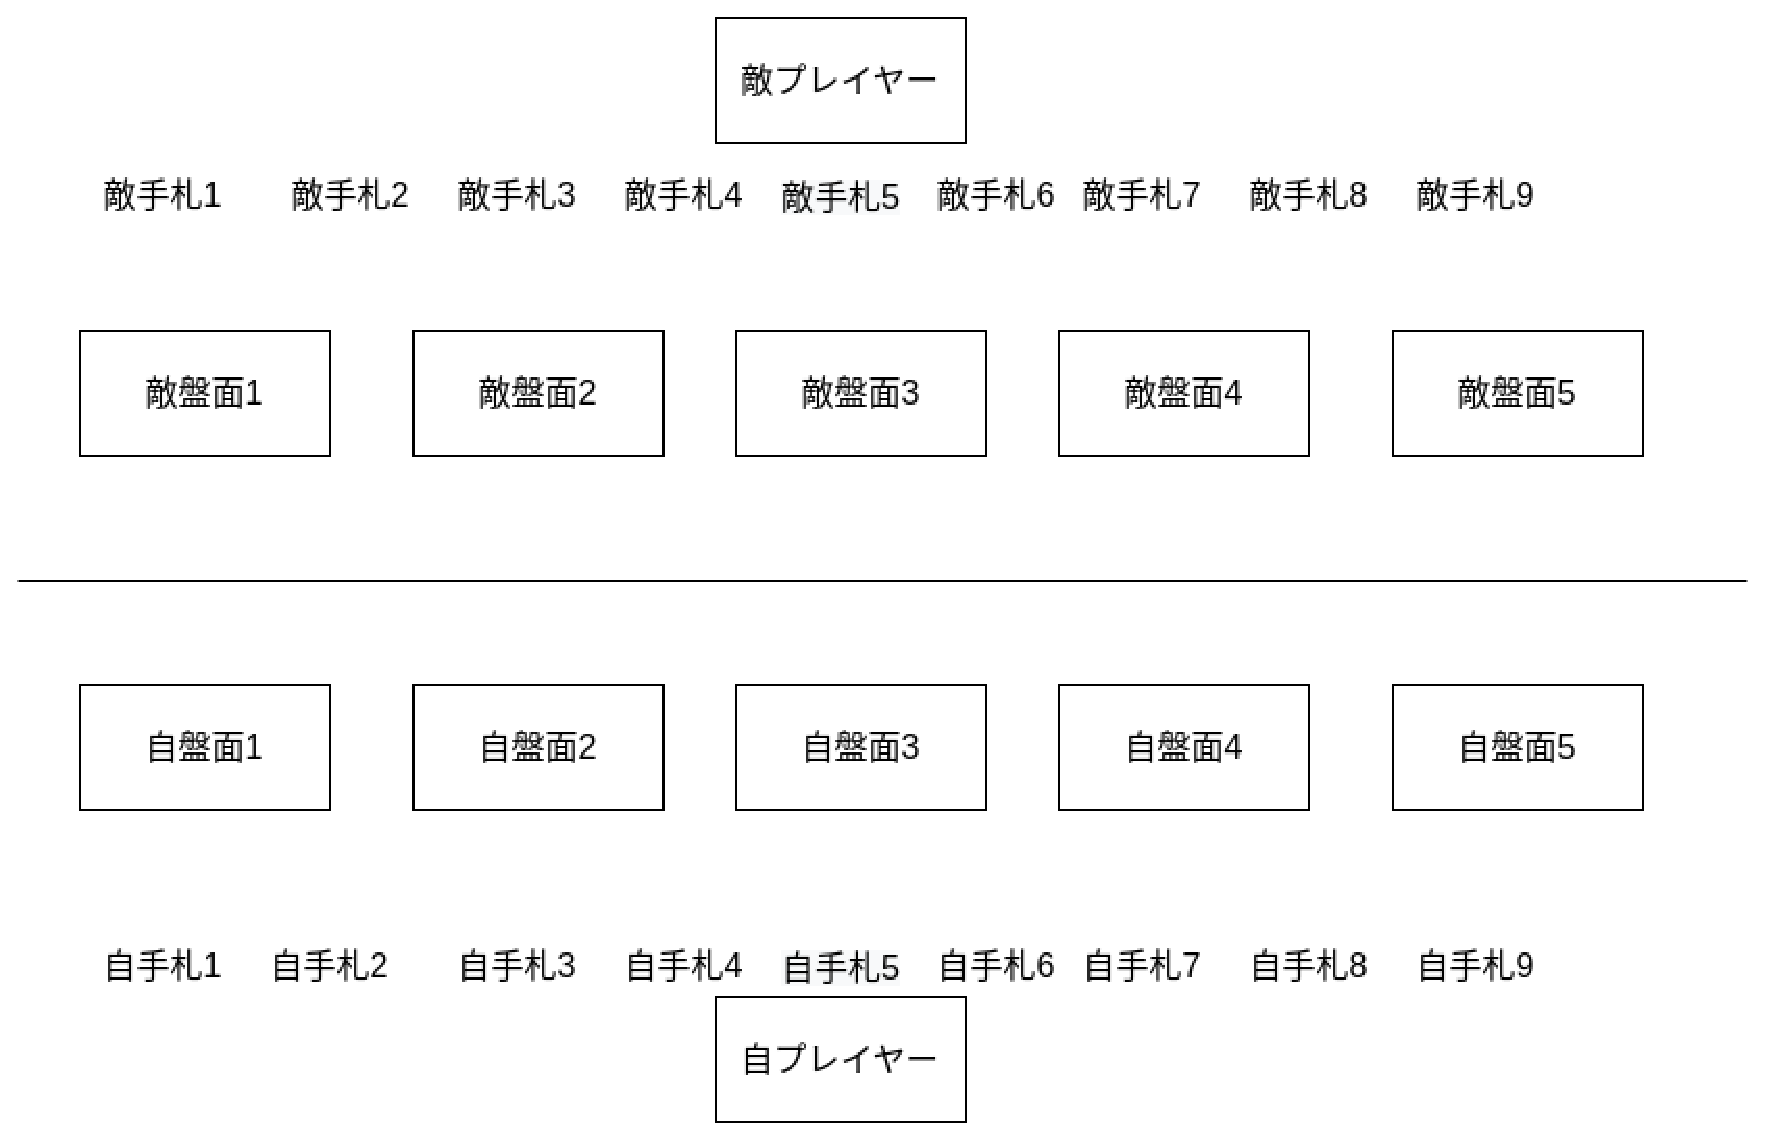
\includegraphics[width=160mm]{assets/idea.eps}
  \caption{作成した環境のイメージ}
  \label{fig:env}
\end{figure}

\begin{table}[H]
  \centering
  \caption{定義した行動空間(太字は今回新規に追加したパラメータ)}
  \label{table:action}
  \begin{tabular}{|c|c|}
  \hline
  行動説明                          & 次元数        \\ \hline
  手札1$\sim$9を自盤面に出す             & 9          \\ \hline
  \textbf{手札1$\sim$9を地盤面に出さない} & \textbf{9} \\ \hline
  自盤面1が敵盤面1$\sim$5に攻撃or何もしない    & 6          \\ \hline
  自盤面2が敵盤面1$\sim$5に攻撃or何もしない    & 6          \\ \hline
  自盤面3が敵盤面1$\sim$5に攻撃or何もしない    & 6          \\ \hline
  自盤面4が敵盤面1$\sim$5に攻撃or何もしない    & 6          \\ \hline
  自盤面5が敵盤面1$\sim$5に攻撃or何もしない    & 6          \\ \hline
  \end{tabular}
  \end{table}

\subsubsection{終了条件の変更}
単純にライブラリ切れで終了すればよい旨のアドバイスを頂いたので反映した.\par
「どちらかのプレイヤーにおいて盤面に盤面にカードが無いかつ手札とデッキにカードが無い場合に終了」
\par
$\Downarrow$
\par
どちらかのプレイヤーが,ライブラリにカードがない時にカードを引こうとした時に終了(ライブラリ切れの時終了)」

\subsubsection{報酬の変更}
現段階ではプレイヤーがターンが回ってくるたびに1枚ドローするルールとなっているためライブラリ切れを勝敗条件に含むと勝率によって学習できているか判断できなくなってしまう.そのため以下のように盤面の残り枚数で設定した.

\begin{equation*}
  reward = 0.0,
  \quad 
  \mathrm{1 エピソード終了後}
  reward \text{ = }
  \left\{
    \begin{aligned}
        1.0 \quad &(自盤面のカード枚数) > (敵盤面のカード枚数) \\
        -1.0 \quad  &(自盤面のカード枚数) \leq (敵盤面のカード枚数)\\
    \end{aligned}
    \right.
\end{equation*}

以前まではエピソード中に報酬を与える検討をしていたためrewardを30としたままだったが,DQNの学習が安定しないという結果を受けて reward cliping として 1.0 と -1.0と報酬を設定した.
\subsubsection{実験1}
上記に示した3つの変更を施して実験した.
モンテカルロ探索で先手,後手ともに 700000 エピソード学習し , 10000 エピソードモデルを検証して勝率を計算した.結果を表 \ref{table:jikken1} に,学習の際のrewardの平均の推移を図 \ref{fig:1First} , \ref{fig:1Second} に示す.

\begin{table}[H]
  \centering
  \caption{実験 1 の結果}
  \label{table:jikken1}
  \begin{tabular}{|c|c|}
  \hline
  学習プレイヤー & 勝率     \\ \hline
  先手      & 0.9344 \\ \hline
  後手      & 0.8562 \\ \hline
  \end{tabular}
  \end{table}

  \begin{figure}[htbp]
    \begin{minipage}[b]{0.52\linewidth}
      \centering
      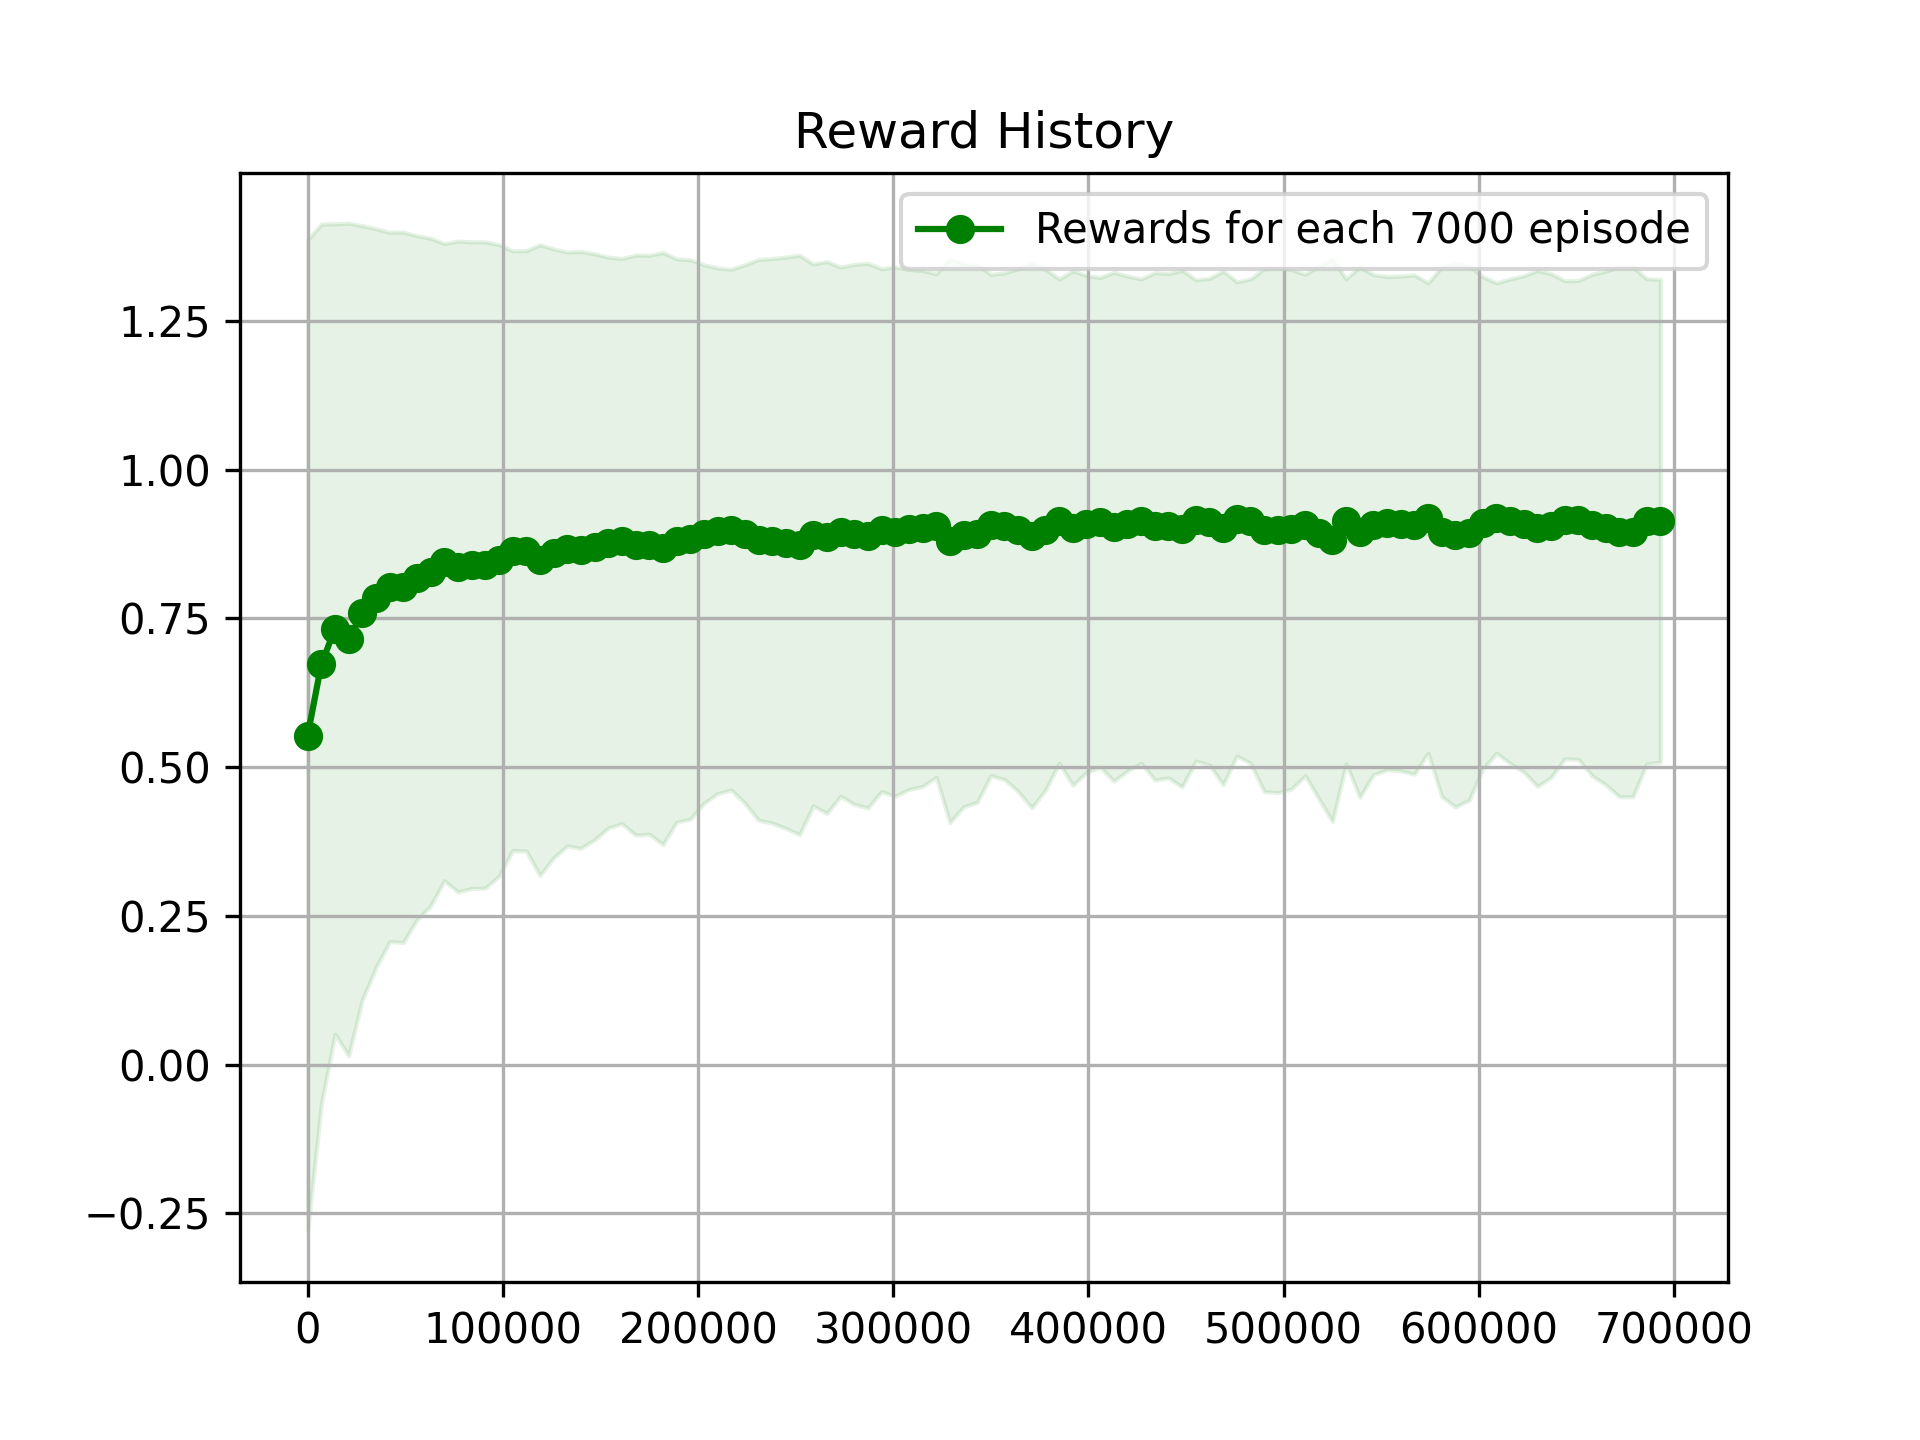
\includegraphics[keepaspectratio, scale=0.60]{assets/MCS700000First.eps}
      \caption{(実験 1 )先手の学習過程における報酬の平均の推移}
      \label{fig:1First}
    \end{minipage}
    \begin{minipage}[b]{0.52\linewidth}
      \centering
      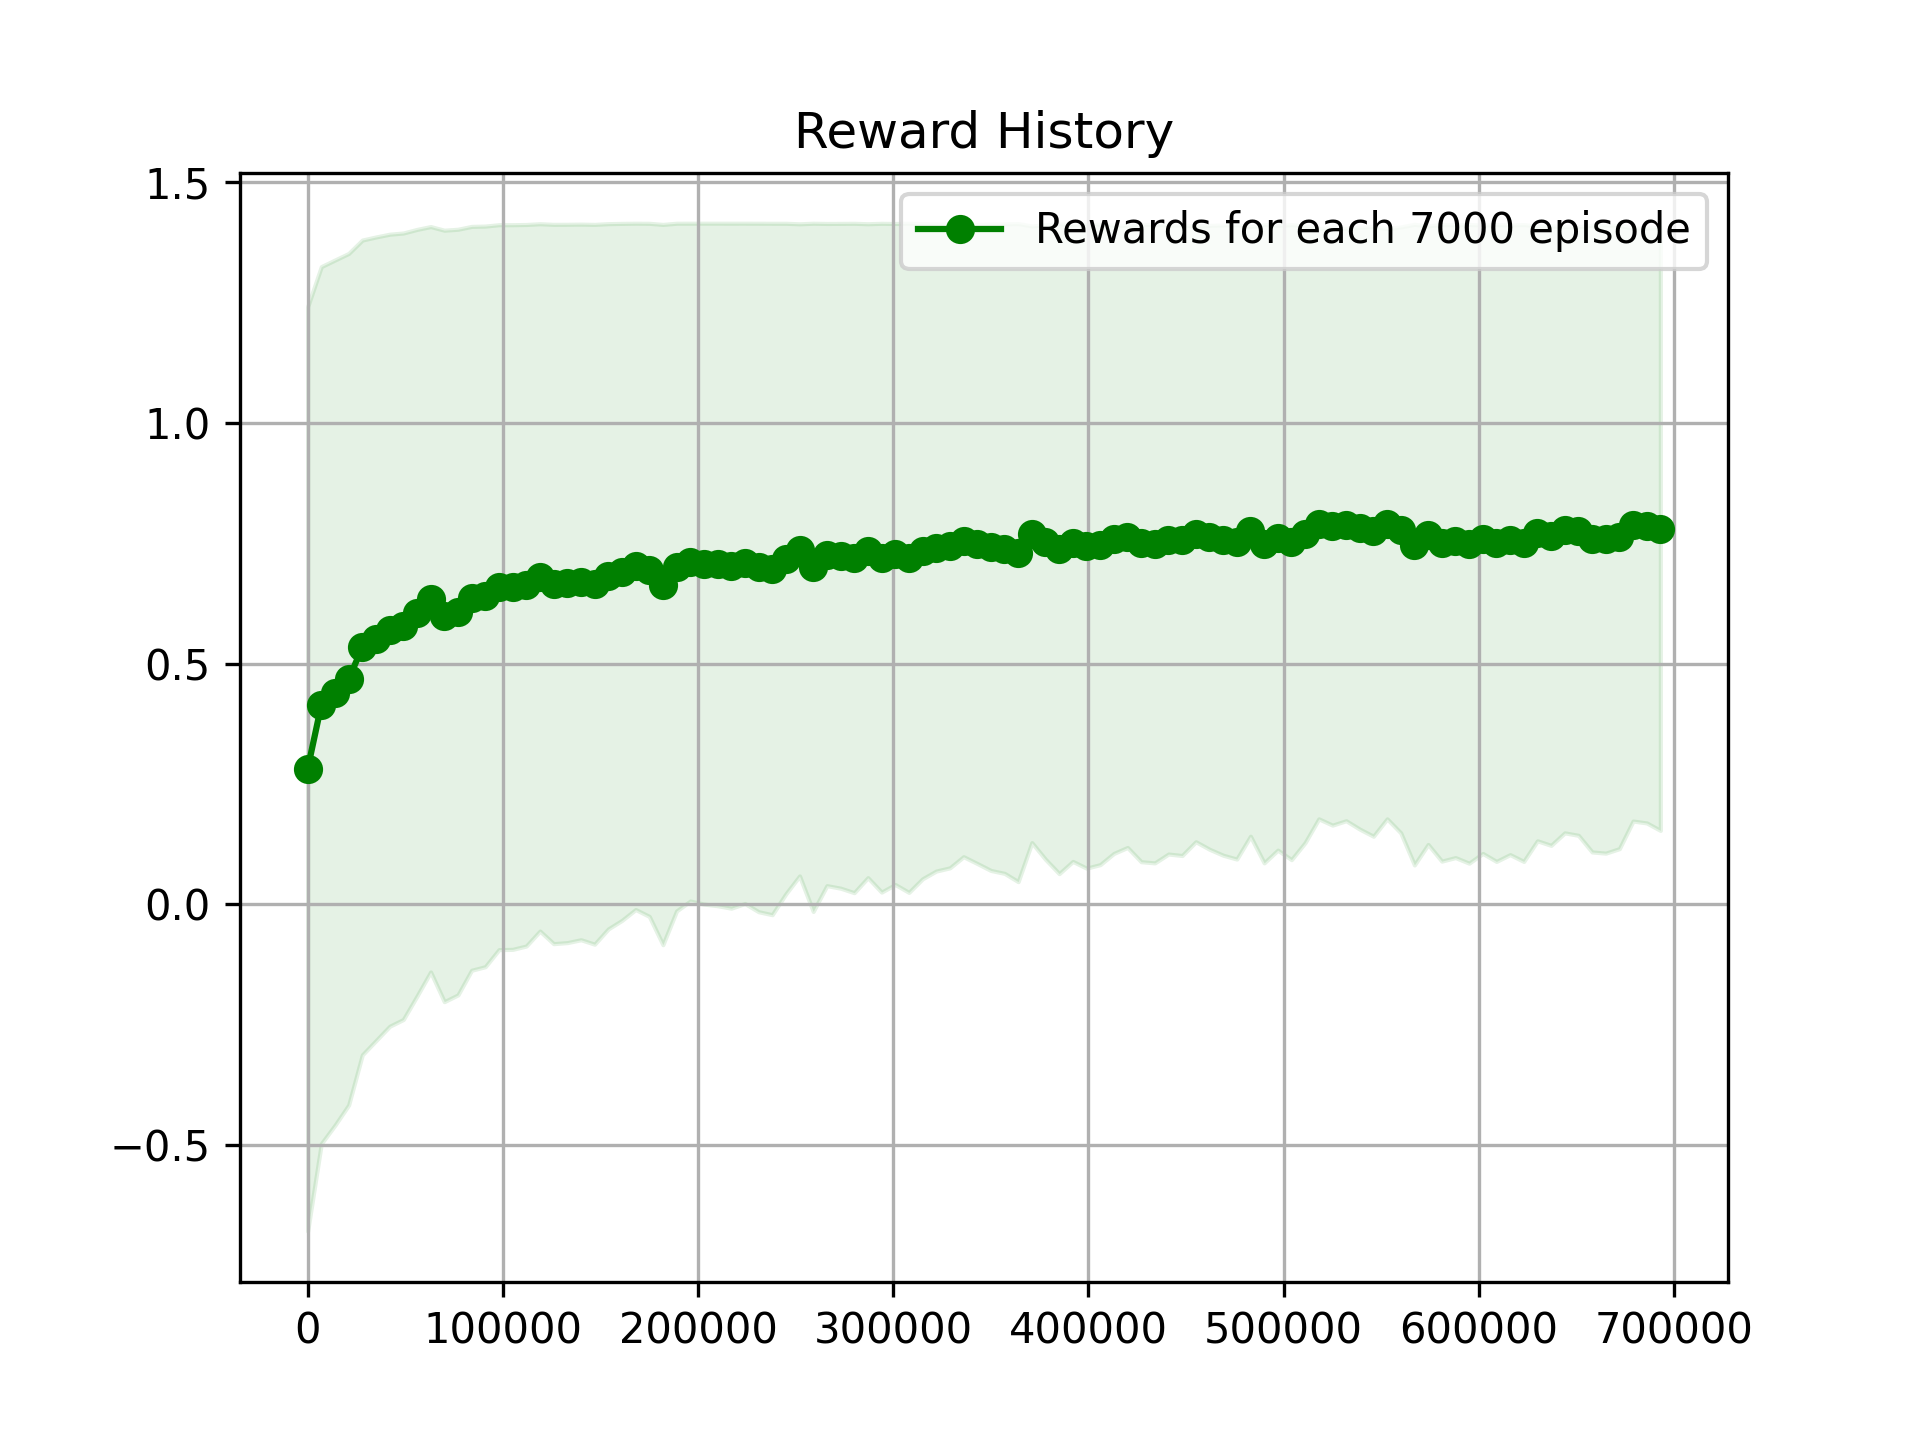
\includegraphics[keepaspectratio, scale=0.60]{assets/MCS700000Second.eps}
      \caption{(実験 1 )後手の学習過程における報酬の平均の推移}
      \label{fig:1Second}
    \end{minipage}
  \end{figure}


\subsubsection{行動空間の定義の変更}
学習する際にライブラリの残り枚数も見れたらゲームエンドまで後何ターンかかるかという状態を含めて学習してくれるのではと考えて行動空間を表 \ref{table:state} のように再定義した.カードが存在しない領域は 0 で Padding している.

\begin{table}[H]
  \centering
  \caption{定義した状態空間 (太字は新しく追加したパラメータ)}
  \label{table:state}
  \begin{tabular}{|c|c|c|c|}
  \hline
  状態説明                        & 次元数        & 最小値        & 最大値         \\ \hline
  手札 1 $\sim$9 の HP と攻撃力      & 18         & 0          & 20          \\ \hline
  自盤面 1 $\sim$5 の HP と攻撃力     & 10         & 0          & 20          \\ \hline
  敵盤面 1 $\sim$5 の HP と攻撃力     & 10         & 0          & 20          \\ \hline
  自盤面 1 $\sim$5 がターン中行動可能かどうか & 5          & 0          & 1           \\ \hline
  \textbf{お互いのライブラリの残り枚数}     & \textbf{2} & \textbf{0} & \textbf{15} \\ \hline
  \end{tabular}
  \end{table}


\subsubsection{実験2}
3.1.5節で述べた行動空間の変更を踏まえて実験 1 と同じ条件で実験した.結果を表 \ref{table:jikken2} ,実験中の報酬の平均の推移を図 \ref{fig:2First}, \ref{fig:2Second}に示す.

\begin{table}[H]
  \centering
  \caption{実験 1 の結果}
  \label{table:jikken2}
  \begin{tabular}{|c|c|}
  \hline
  学習プレイヤー & 勝率     \\ \hline
  先手      & 0.9435 \\ \hline
  後手      & 0.8589 \\ \hline
  \end{tabular}
  \end{table}

  \begin{figure}[htbp]
    \begin{minipage}[b]{0.52\linewidth}
      \centering
      \includegraphics[keepaspectratio, scale=0.60]{assets/2First.eps}
      \caption{(実験 2 )先手の学習過程における報酬の平均の推移}
      \label{fig:2First}
    \end{minipage}
    \begin{minipage}[b]{0.52\linewidth}
      \centering
      \includegraphics[keepaspectratio, scale=0.60]{assets/2Second.eps}
      \caption{(実験 2 )後手の学習過程における報酬の平均の推移}
      \label{fig:2Second}
    \end{minipage}
  \end{figure}

ランダム性を考慮すると有意な勝率の増加とは言えない程度であるが,勝率は向上している.採用しない理由もないため,状態空間の定義にライブラリの残り枚数も加えることとする.

\subsection{モデル側の改善}
DQN は keras のライブラリを使用して実装していた.そのため細かいチューニングは難しいが,提供されているパラメータを調整し表 \ref{table:modelpram} のように改善を試みた\cite{DQNparam}.

\begin{table}[H]
  \centering
  \caption{実験 1 の結果}
  \label{table:modelpram}
  \begin{tabular}{|c|c|c|}
  \hline
  変更したパラメータ                      & 変化前  & 変化後   \\ \hline
  Experience Memoryへの書き込み開始ステップ数 & 1000 & 10000 \\ \hline
  Target Network の更新重み           & 0.01 & 0.5   \\ \hline
  \end{tabular}
  \end{table}

\subsubsection{Exprience Memoryへの書き込み開始Stepの調整}
keras-rl には nb\_steps\_warmup というパラメータが存在し, Exprience Memory への書き込みを nb\_steps\_warmup ステップ終わってから始めることで学習が進んで無い場合の不安定な状態をExprience Memory に書き込むことを防いでいる. 標準は 1000 ステップとなっていたため 10000 ステップへと変更した.また,Exprience Memoryのメモリ量を 1000000 から 50000 に変更した.

\subsubsection{Target Network の更新の重み調整}
keras-rl は 1 ステップごとに target\_model\_update というパラメータで, \par
target\_model = target\_model\_update * target\_model + (1 - target\_model\_update) * model
\par
という式でTarget Networkのパラメータの更新を行っている.
 DQN において Q 値の更新式の $maxQ(s_{t+1},a_{t+1})$ の計算で Target Network が用いられている\cite{targetnetwork}.標準では $1e-2$ となっていたが, DQN がステップを重ねても学習が進まなかったことを考え 0.5 とした.

\section{実験 3}
DQN で 5000000 ステップ学習を行い, 学習したモデルを 10000 回検証し勝率を検証した. その後,同程度エピソード数モンテカルロ探索で学習・検証を行い勝率を比較した.なお,学習プレイヤーは後手とした.DQN のパラメータを表 \ref{table:updateparam} に示す.
結果を表 \ref{table:jikkenDQN} ,学習過程での100エピソードの報酬の平均の推移を図 \ref{fig:3DQN}, \ref{fig:3MCS} に示す.

\begin{table}[H]
  \centering
  \caption{DQNのパラメータ}
  \label{table:updateparam}
  \begin{tabular}{|c||c|}
  \hline
  方策                 & ε-greedy \\ \hline
  ε                      & 0.1      \\ \hline
  全結合層の活性化関数             & ReLU     \\ \hline
  全結合層の次元                & 64       \\ \hline
  最適化アルゴリズム              & Adam     \\ \hline
  Target Network 更新重み              & 0.5     \\ \hline
  Exprience Memory への書き込み開始step & 10000 \\ \hline
  Experience Replayのメモリ量 & 50000  \\ \hline
  \end{tabular}
  \end{table}

\begin{table}[H]
  \centering
  \caption{実験 3 の結果}
  \label{table:jikkenDQN}
  \begin{tabular}{|c|c|}
  \hline
  method & 勝率     \\ \hline
  DQN      & 0.9069 \\ \hline
  MCS      & 0.7257 \\ \hline
  \end{tabular}
  \end{table}

  \begin{figure}[H]
    \begin{minipage}[b]{0.52\linewidth}
      \centering
      \includegraphics[keepaspectratio, scale=0.60]{assets/5000000DQN.eps}
      \caption{(実験 3 )DQNにおける報酬の平均の推移}
      \label{fig:3DQN}
    \end{minipage}
    \begin{minipage}[b]{0.52\linewidth}
      \centering
      \includegraphics[keepaspectratio, scale=0.60]{assets/85000MCS.eps}
      \caption{(実験 3 )MCSにおける報酬の平均の推移}
      \label{fig:3MCS}
    \end{minipage}
  \end{figure}

100エピソードでの報酬平均をとってしまったので見辛いグラフとなったが, DQN が学習できていることが分かる.



\section{HP, コスト, 特殊効果をつけたverの環境作成}
DQN の学習時間がかなり長かったので今後の環境の拡張も考え実装した.
作成した特殊効果は以下の通りである.
\begin{quote}
  \begin{itemize}
   \item 盤面に出したら (攻撃力 , HP) = ( 1 , 1 )のユニット追加で出す.
   \item 盤面に出したら自プレイヤーの HP を 2 回復
   \item 盤面に出したら敵プレイヤーの HP を 2 削る
   \item 盤面に出したら自プレイヤーは 1 枚カードをドロー
   \item 盤面に出たターンに攻撃できる
  \end{itemize}
 \end{quote}


\section{今後の課題}
\begin{quote}
  \begin{itemize}
   \item 来週の発表練習,再来週の発表について
   \par
   テーマは「自作カードゲーム環境における強化学習手法の適用の検討」と考えています.ですが,今まで改善⇔実験の繰り返ししかしてないためどのような発表にすればよいか悩んでいます. 本資料のように「こういう問題が生まれたのでこういう対処をしたら上手く行った」といった形式で発表になるのでしょうか.

   \item これからの方針について
   \par
   先週も同じこと言ってたんですが,ここからどのように卒研に落とし込むかの方針が立っていません.自作環境で既存手法試すことが卒研のハードルを満たしているなら,AlphaZero や Rainbow といった現在実装済みのアルゴリズムの上位互換,またReBeL\cite{ReBeL}, MuZero\cite{MuZero}, DreamerV2\cite{DreamerV2} といった最近考案された不完全情報ゲームに対する手法を実装して検証してみたいと思っているのですが難易度が高いかつ新規性が薄いのではないかと感じています.恐縮ですがお時間があれば相談したいです.

   \item 学習したモデル同士を戦わせるようにする
   \par
   勝率の比較だとモデルの優劣を厳密に示せないため作成したい

   \item 可視化シュミレータ
   \par
   必要性は薄いかもしれないが,実験の結果を可視化できるようになれば考察や発表の際役に立ちそう.PyGame は触ったこと無いので Unity でログ食わせる方法になりそう.
  \end{itemize}
 \end{quote}

%index.bibはtexファイルと同階層に置く
%ちゃんと\citeしないと表示されない(1敗)
\bibliography{index.bib}
\bibliographystyle{junsrt}

\end{document}